% ===========================================================================
\section{Extension: two-point functions}\label{sec:twopoint}
% ===========================================================================

Power spectra are the natural output of a Boltzmann code, because each Fourier mode or multipole evolves
independently in linear theory. Observers often measure the equivalent real-space two-point functions instead. They
show localized features, such as the acoustic scale or the BAO peak, as features at one separation, and they are
easier to estimate on a masked sky or in a survey with complicated geometry. We added functions that compute the
angular correlation functions of the CMB, the three-dimensional correlation function of the matter, and the angular
power spectrum and correlation function of the matter (or galaxy) density projected over a redshift distribution.

\subsection{Theory}

\paragraph*{Angular correlation functions.} For a statistically isotropic field on the sphere,
$a_{\ell m}$ are uncorrelated with variance $C_\ell$, and the addition theorem
$\sum_mY_{\ell m}(\hat n)Y^*_{\ell m}(\hat n')=\frac{2\ell+1}{4\pi}P_\ell(\hat n\cdot\hat n')$ gives
\begin{equation}
C(\theta)=\langle T(\hat n)T(\hat n')\rangle=\sum_\ell\frac{2\ell+1}{4\pi}C_\ell B_\ell^2P_\ell(\cos\theta),
\label{eq:Ctheta}
\end{equation}
with an optional Gaussian beam $B_\ell=e^{-\ell(\ell+1)\sigma_b^2/2}$. The polarization is a spin-2 field, so its
correlation functions involve the Wigner functions $d^\ell_{mm'}$ of Sec.~\ref{sec:lensing}. With $Q$ and $U$ measured
relative to the great circle joining the two points~\cite{Challinor2005},
$\xi_\pm=\langle QQ\rangle\pm\langle UU\rangle=\sum_\ell\frac{2\ell+1}{4\pi}(C_\ell^{EE}\pm C_\ell^{BB})d^\ell_{2,\pm2}$
and $\xi_X=\langle TQ\rangle=\sum_\ell\frac{2\ell+1}{4\pi}C_\ell^{TE}d^\ell_{20}$. We sum
$\ell=2$--2500 (the monopole and dipole are not cosmological) with the Legendre and Wigner recurrences.

\paragraph*{Matter correlation function.} In three dimensions the transform is
\begin{align}
\xi(r)&=\int_0^\infty\frac{k^2dk}{2\pi^2}P(k)j_0(kr)\nonumber\\
&=\frac{1}{2\pi^2r}\int_0^\infty dk\,kP(k)\sin(kr).
\end{align}
The integrand oscillates many times for $r\sim100\Mpc$, so we use Filon's method~\cite{Filon1929}: $kP(k)$ is
interpolated linearly in $k$ between tabulated points and the product with $\sin(kr)$ is integrated analytically. The
grid then only has to resolve $P(k)$, including its BAO wiggles (we use $d\ln k=0.002$ and $dk\le5\times10^{-4}\Mpc^{-1}$
below $1\Mpc^{-1}$), for all $r$ at once. The integral needs $P(k)$ up to $k\sim10\Mpc^{-1}$. Beyond the computed range
we extrapolate $\Delta_M\propto k^2T(k)$ with the shape of the no-wiggle transfer function of
Ref.~\cite{EisensteinHu1998} anchored at $k_{\max}$ (accurate to 1.5\% up to $20\Mpc^{-1}$ from $k_{\max}=0.3\Mpc^{-1}$),
and $\Delta_M\propto k^2$ below $k_{\min}$. We also compute $\sigma_R$, the rms of $\Delta_M$ in top-hat spheres, and
$\sigma_8$.

\paragraph*{Projected density.} A galaxy survey with redshift distribution $n(z)$ and linear bias $b$ sees the
projected field $\delta_g(\hat n)=\int d\chi\,W(\chi)\,b\,\Delta_M(\chi\hat n,\chi)$ with $W=n(z)\,dz/d\chi$ normalized to
unit integral. Expanding the plane waves in spherical harmonics, as for the CMB (Sec.~\ref{sec:m4}),
\begin{align}
C_\ell&=4\pi\int\frac{dk}{k}\mathcal P_{\mathcal R}(k)\Delta_\ell(k)^2,\nonumber\\
\Delta_\ell(k)&=\int d\chi\,W(\chi)\,b\,\Delta_M(k,\chi)\,j_\ell(k\chi).
\label{eq:clgal}
\end{align}
For $\ell\gg1$, $j_\ell(k\chi)$ picks out $k\chi\approx\ell+\frac12$, and Eq.~\eqref{eq:clgal} reduces to the Limber
approximation~\cite{Limber1953,LoVerde2008},
$C_\ell=\int d\chi\,W^2b^2P((\ell+\frac12)/\chi,\chi)/\chi^2$: the multipole $\ell$ probes the transverse wavenumber
$k=(\ell+\frac12)/\chi$ at each distance. The Limber approximation drops the radial modes, which matter when the window is
not much wider than the wavelength. For $\sigma_z=0.1$ at $z=1$ it is 4\% wrong at $\ell=20$ and 0.4\% at $\ell=100$, so we
use the exact projection below $\ell=200$ (with all $j_\ell$ for one $k\chi$ from a single recurrence) and Limber
above. We include only the density term: redshift-space distortions, lensing magnification and the relativistic
corrections are left out, and $P(k)$ is linear. The angular correlation function $w(\theta)$ follows from
Eq.~\eqref{eq:Ctheta}; small angles need $\ell$ up to $\sim3\times10^4$ (Limber on a logarithmic grid, with a cosine
taper at the end to avoid ringing from the truncation).

\begin{figure*}
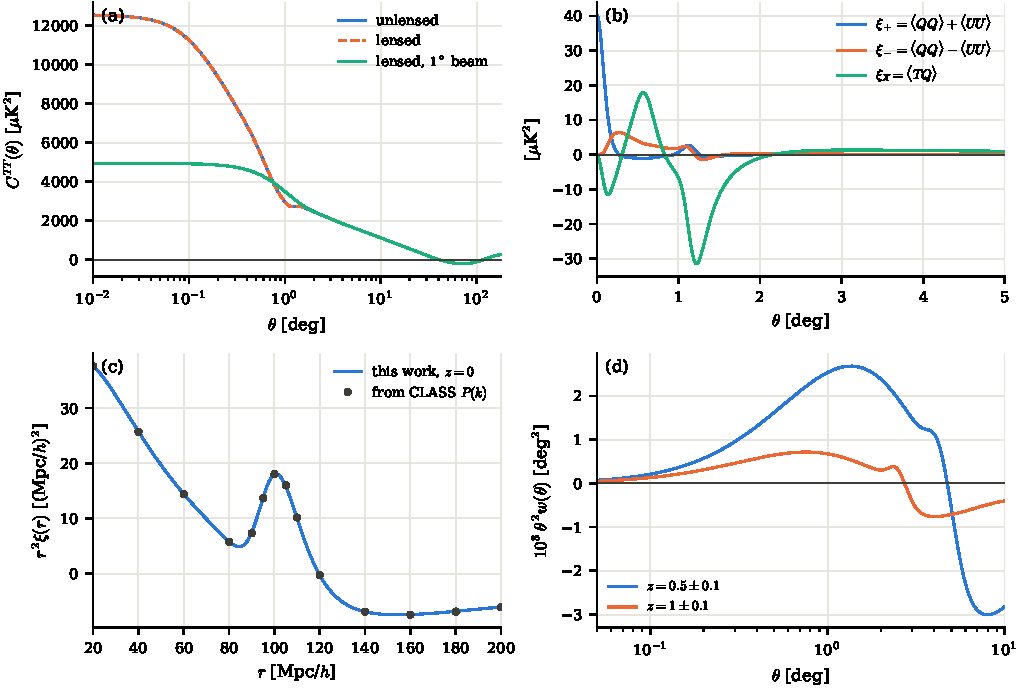
\includegraphics[width=0.95\textwidth]{twopoint}
\caption{Two-point functions of the fiducial model. \emph{(a)} CMB temperature correlation function, unlensed,
lensed, and lensed with a $1^\circ$ beam. \emph{(b)} Polarization correlation functions (unlensed). \emph{(c)}
Matter correlation function today, with the BAO peak; points are the transform of CLASS's $P(k)$. \emph{(d)} Angular
correlation function of the matter projected over Gaussian redshift distributions ($\sigma_z=0.1$, $b=1$).}
\label{fig:twopoint}
\end{figure*}

\subsection{Results}

\paragraph*{CMB.} The variance of the temperature is $C(0)=12\,550\muK$, i.e.\ $112\,\mu$K rms (Fig.~\ref{fig:twopoint}a).
The correlation falls to half at $\theta\approx0.5^\circ$, the angle subtended by the scales of the first acoustic peak,
and shows a shoulder near $1^\circ$. This is the real-space counterpart of the acoustic peaks: the sound horizon
subtends $\theta_*=r_s/\chi_*=0.60^\circ$, and a localized initial perturbation produces a ring of that radius around
itself. At large angles $C(\theta)$ is set by the lowest multipoles. It crosses zero at $41^\circ$ and $117^\circ$, with
$-205\muK$ at $72^\circ$ and $+259\muK$ at $180^\circ$. Because only a few multipoles contribute, the cosmic variance
of $C(\theta)$ is large here; the observed sky shows almost no correlation above $60^\circ$, one of the known
large-angle anomalies. Lensing changes $C(\theta)$ by at most $6\muK$ (at $1.1^\circ$, where it smooths the acoustic
shoulder), and conserves the variance to $10^{-4}$, since it only remaps the sky. A $1^\circ$ beam reduces the variance
to $4\,940\muK$. The polarization has rms $\sqrt{\xi_+(0)}=6.3\,\mu$K (Fig.~\ref{fig:twopoint}b). The
temperature--polarization correlation $\xi_X$ is $+18\muK$ at $0.57^\circ$ and $-31\muK$ at $1.22^\circ$: around a
temperature hot spot the polarization alternates between radial and tangential. This pattern comes from the flow of
the photon--baryon fluid into and out of the potential wells at decoupling, and it has been seen by stacking hot
spots in the WMAP data~\cite{Komatsu2011}.

\paragraph*{Matter.} The matter correlation function (Fig.~\ref{fig:twopoint}c) has the BAO peak at
$r=100.5\,h^{-1}\Mpc=150\Mpc$, close to the sound horizon at the drag epoch, $r_d=147\Mpc$ (the smooth decline of
$\xi$ moves the maximum of $r^2\xi$ slightly outward). Each initial point perturbation launches a spherical sound wave
in the photon--baryon fluid that stalls at $r_d$ when the baryons are released, so the baryons, and the dark matter
that later falls into them, end up with a shell at $r_d$ around every overdensity~\cite{Eisenstein2005}. In Fourier
space this single feature appears as the series of BAO wiggles. We find $\sigma_8=0.82071$ (CLASS: 0.82068). Our
$\xi(r)$ agrees with the transform of CLASS's $P(k)$ (computed independently with adaptive quadrature) to
$3\times10^{-4}$ at $r=20\,h^{-1}\Mpc$, and to 0.9\% of the BAO peak height of $r^2\xi$ for $r\ge60\,h^{-1}\Mpc$. The
latter is not numerical, as the transform reproduces analytic and quadrature results to $10^{-6}$ and $7\times10^{-4}$ in
the unit tests. It comes from the $\pm7\times10^{-4}$ oscillating difference between the two $P(k)$, which follows
the BAO phase (Sec.~\ref{sec:validation}): the BAO peak in $\xi$ is a small residual of a large cancellation, and it is
sensitive to the damping and phase of the wiggles.

\paragraph*{Projected density.} For Gaussian redshift distributions at $z=0.5$ and 1 ($\sigma_z=0.1$), our $C_\ell$ agree
with CLASS's number-count spectra (density term only, exact projection) to $7\times10^{-4}$ and $1.7\times10^{-3}$ for
$\ell\le500$, and to $1.9\times10^{-3}$ for $500<\ell\le2000$ (computed with $k_{\max}=1\Mpc^{-1}$; with the default
$0.3\Mpc^{-1}$ the extrapolated $P(k)$ misses the residual BAO wiggles, which costs up to 1.5\% at $\ell=1000$--2000). In $w(\theta)$
(Fig.~\ref{fig:twopoint}d) the BAO shell appears at the angle $r_d/\chi(z)$. For $z=1$ we find the feature at
$2.36^\circ$, against $r_d/\chi=2.47^\circ$; projection smooths it into a shoulder that ends at this angle, since pairs
at different distances along the line of sight have transverse separations below $r_d$. For $z=0.5$ the expected angle,
$4.3^\circ$, is close to where $w$ changes sign, and the feature is hard to see. The correlation is weaker at higher
redshift because the structure is younger (growth factor) and a fixed angle corresponds to a larger physical scale.
